\providecommand{\rasd}{..}
\documentclass[../RASD.tex]{subfiles}

\begin{document}
    \chapter{Architectural Design}\label{ch:architectural-design}
    \section{Overview}\label{sec:overview}
    From an external point of view, users using their smartphones, exploits the different services offered by SafeStreets that are different for citizen and authority.

    The application to be developed is based on one application component ( application logic) which manages the interactions between different components of the system.

    Application logic is present both in the mobile view and in the back-end logic.
    In mobile view there is the management of the GUI and of the connection with other useful components present in the smartphone: GPS and camera;
    while in the back-end logic there is the most of the logic and also the interfaces to external services:
    Database provider, Plate recognition provider, map provider and authentication provider.
    \begin{figure}[H]
        \centering
        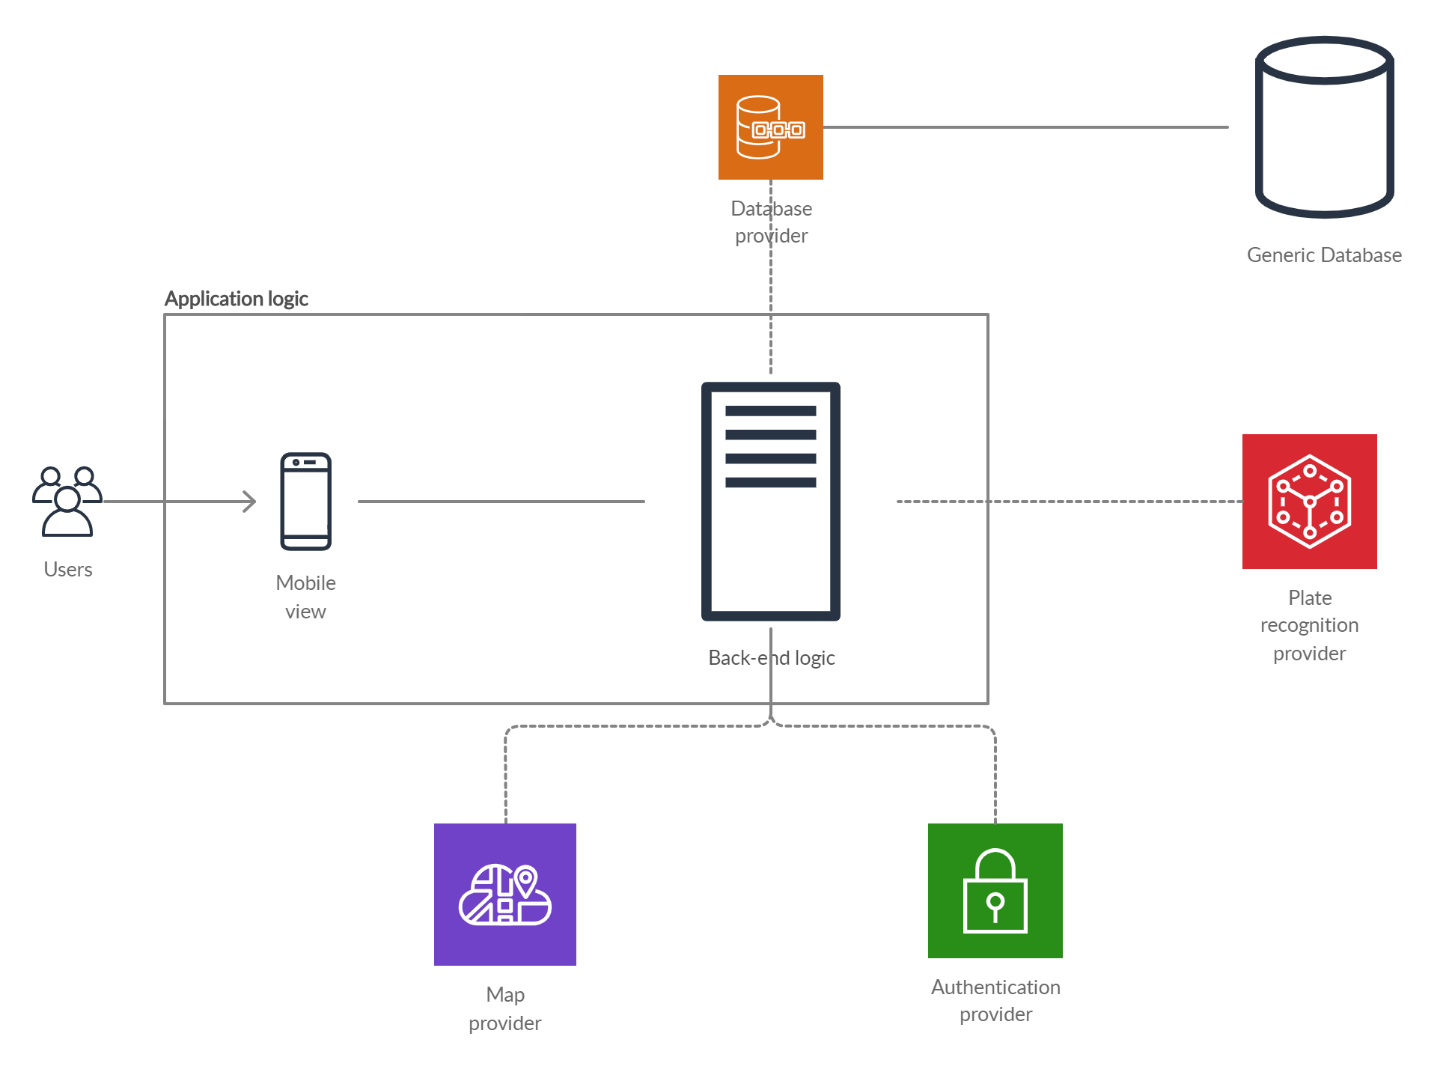
\includegraphics[scale = 1.3]{assets/overview.png}\\[1.6 cm]
        \caption[\textit{OverView} Diagram]{Overview diagram of the application.}
    \end{figure}
    \section{Component View}\label{sec:component-view}
    \begin{figure}[H]
        \centering
        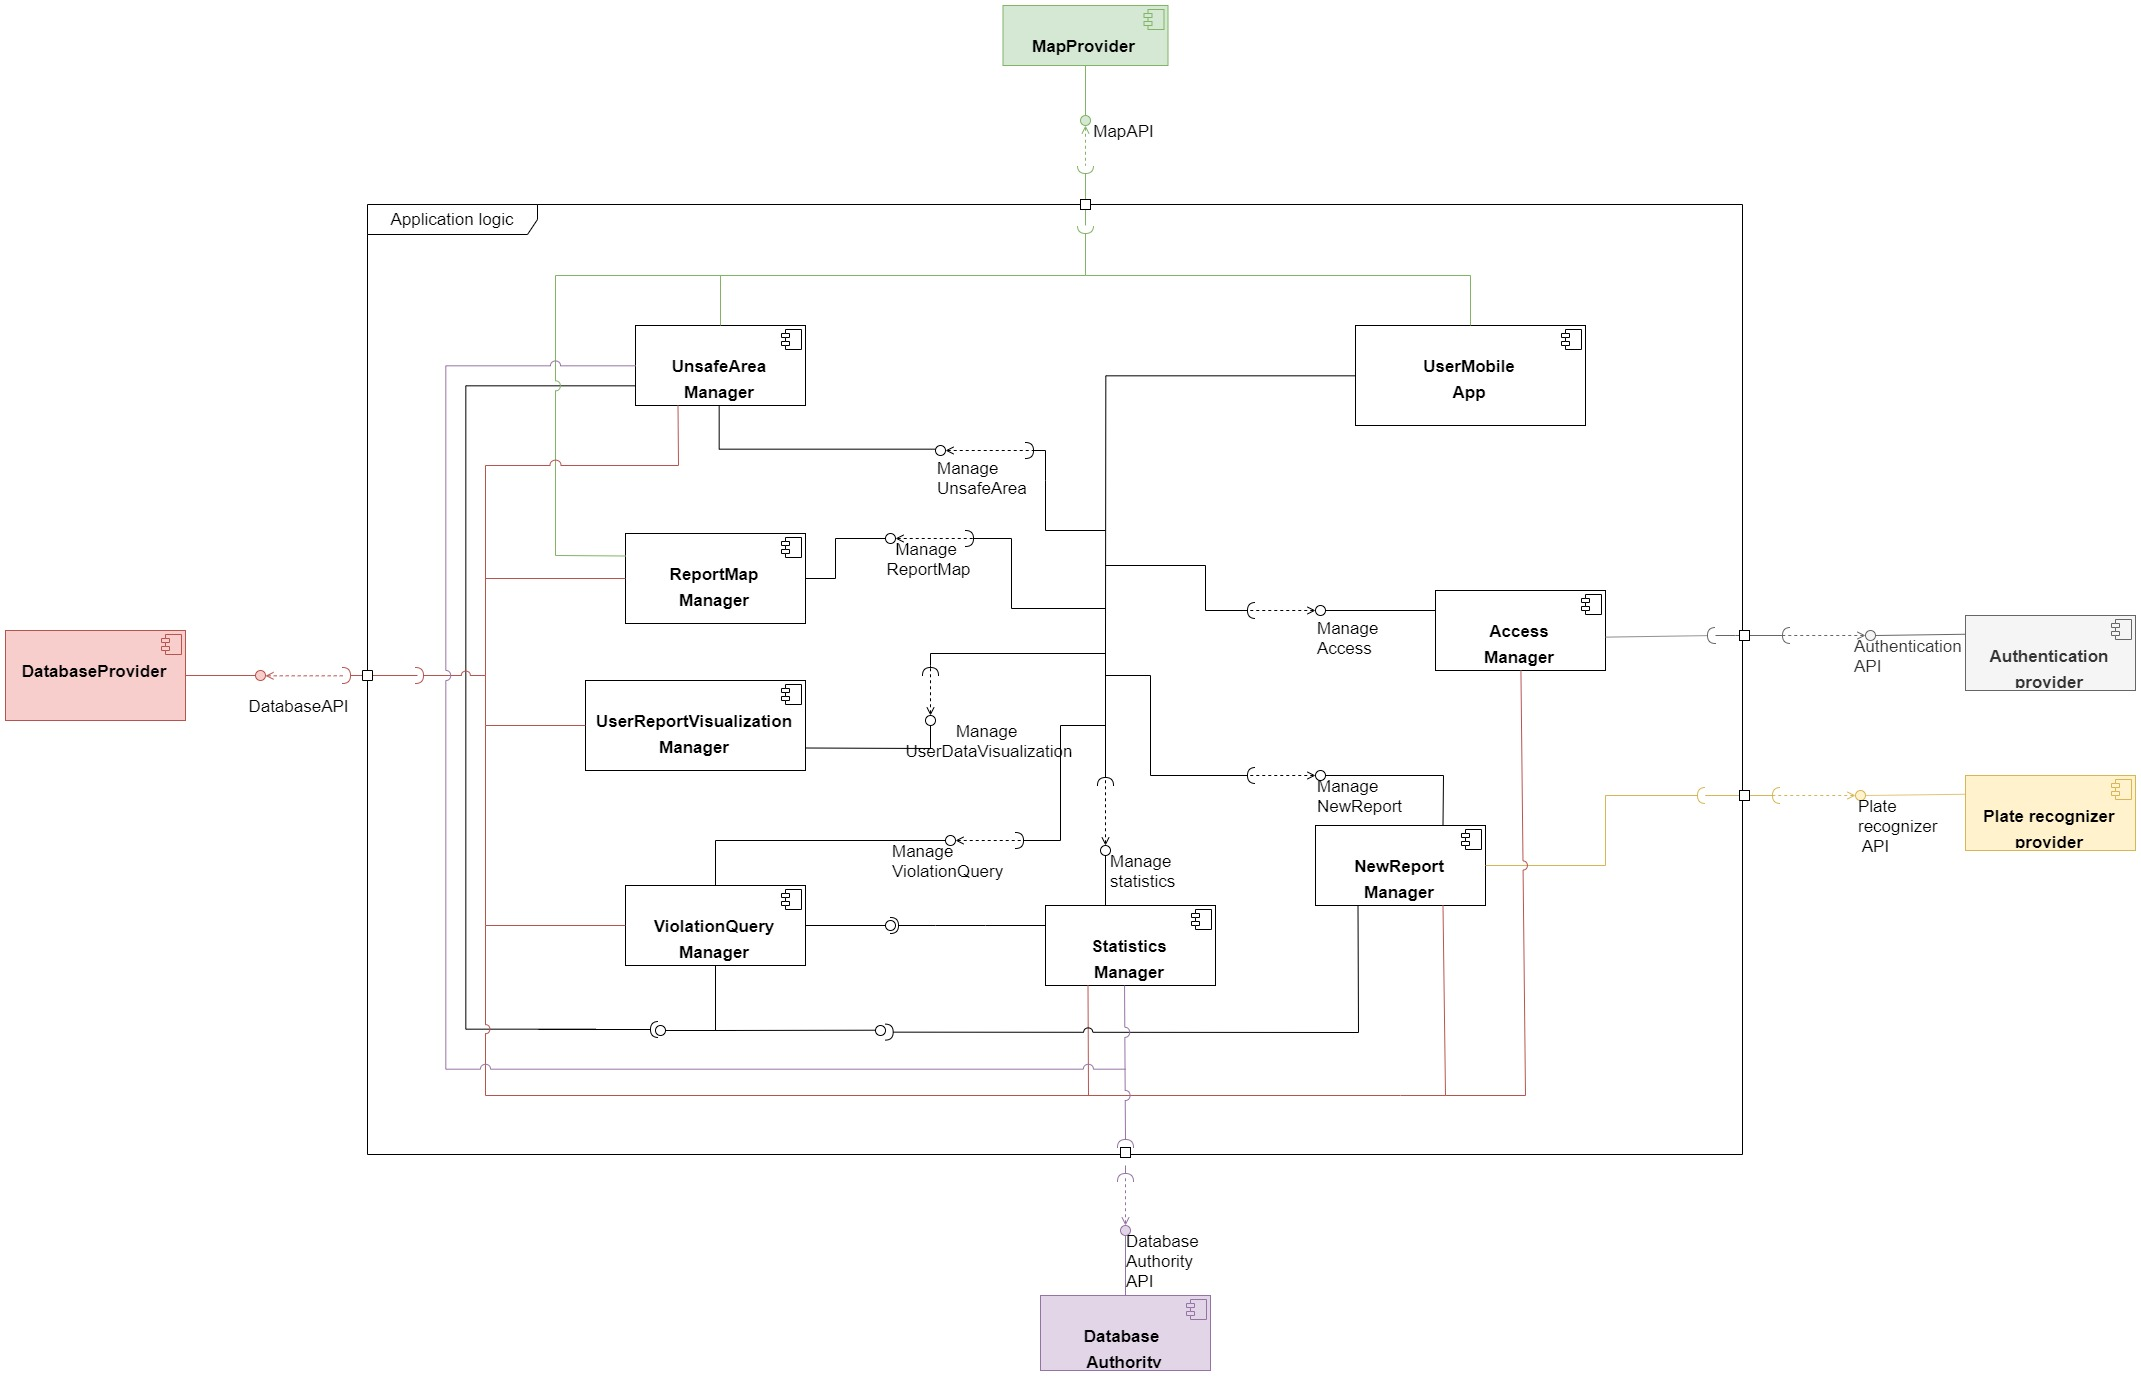
\includegraphics[scale = 0.24]{assets/component.png}\\[1.6 cm]
        \caption[\textit{Component} Diagram]{Component diagram of the application.}
    \end{figure}
    The components’ functions contained in the application are described in the following list:
    \begin{itemize}
        \item \textbf{ReportMap Manager:} it takes care of showing on the map all the report with the correct color of pointer.
        It does that using the position of the report retrieved by gps on device.
        It interacts with map provider to shows all the reports in the correct position and also with database provider to retrieve the report position.
        Furthermore if a user clicks on a pointer of a report, this manager shows all the information of selected report concerning the type of user:
        if a citizen the plate are obscured otherwise they aren’t.
        \item \textbf{NewReport Manager:} it manages the insertion of a new report: procedures to validate the correctness and completeness of the report
        and to retrieve the position of the user using the gps on the device.
        It interacts with plate recognizer provider to recognizes the plate in the image so this manager can obscure the position of the plate it the picture.
        It checks if there is a report of same type, in the same position and at the same date (using violationQuery manager)
        and the manager sends the report to the database provider which stores it.
        \item \textbf{Access Manager:} it manages the sign up and login of the users.
        In particular, it interacts with authentication provider (which contains all the procedures to register a new customer and to authenticate a registered one).
        For the sign up of an authority is mandatory insert not only mail address and a password but also the ID\@.
        Access manager also interacts with database provider on which there are stored the mails of the users.
        This is useful for keep an association between the user and all his reports.
        \item \textbf{UserReportVisualization Manager:} it manages the visualization of all reports of one user.
        In particular interacts with database provider from which takes reports stored.
        It shows all the reports of a user and also the possible actions on it: delete, modify, feedback area and only for authority
        it displays the field to check if a report is used to generate a traffic tickets.
        \item \textbf{ViolationQuery Manager:} it manages all the procedures to make a query on the database (through the database provider)
        to retrieve same specific data.
        User, unsafeArea manager, statistics manager and also NewReport manager use violationQuery manager to obtain data.
        Users have a dedicated area in the application where they can make a query by setting different fields (data, type, zone).
        UnsafeArea manager uses it to retrieve information in this way can fins unsafe area.
        Statistics manager use violationQuery manager to build statistics on the reports and the NewReport manager checks correctness of a report
        that is going to be add by checking position and data of report already stored in the database.
        \item \textbf{Statistics Manager:} it takes care of building statistics on the app through specific algorithms.
        It retrieves data using both database provider in which are stored data about reports and databases of authority in which are stored data about accidents.
        In particular it builds statistics on effectiveness of the application analyzing the feedback by authority (reports used for generate traffic tickets)
        and on the crimes.for all type of statistics, this manager checks if there is at least one user from which it takes data.
        \item \textbf{UnsafeAreaManager:} it takes care of showing on the map the unsafe areas.
        It, using services provided by violationQuery manager and also data from the authority database,
        finds unsafe areas and it displays on the map information retrieved.
        Furthermore only for authorities it show suggestions for possible intervention in that specific area.
        \item \textbf{UserMobile App:} it’s the application on users devices, it interacts with all the services provided by the different managers,
        it also exploits the map provider on which there are all reports with their own position.
        It takes the user interaction and feedback.
        It manages GUI and also the permission of the user to use the GPS and the camera.
    \end{itemize}

    \textbf{Providers:}
    \\
    \begin{itemize}
        \item \textbf{Plate Recognition Provider:} it is used to recognize the plate of a car from a picture loaded by a user.
        \item \textbf{Map Provider:} it provides a real time map of the globe.
        \item \textbf{Authentication Provider:} it manages the access of a registered users and the registration of new one.
        \item \textbf{Database Provider:} it is used to store all the information regarded the reports and the user information.
    \end{itemize}
    \textbf{Other Components:}
    \\
    \begin{itemize}
        \item \textbf{Database Authority:} it is used by SafeStreets in particular w.r.t component diagram, unsafeArea manger and statisticsManager
        exploit it to use data about accidents.
    \end{itemize}
    \section{Deployment View}\label{sec:deployment-view}
    In the following image the SafeStreets deployment diagram is represented: it shows the execution architecture of the system
    and represents the distribution (deployment) of software artifacts to deployment targets (nodes).
    Artifacts, in general, represent pieces of information that are used or are produced by a software development process and are deployed on nodes
    that can represent either hardware devices or software execution environments.
    \begin{figure}[H]
        \centering
        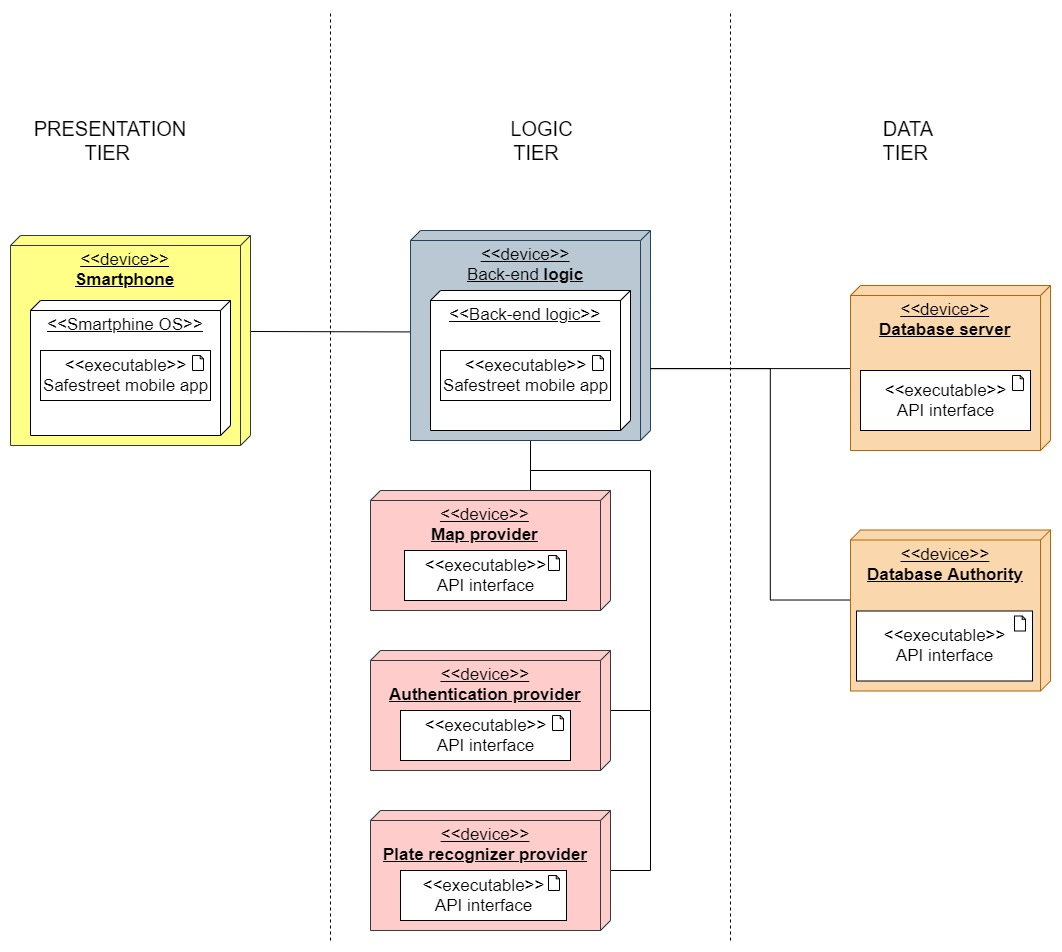
\includegraphics[scale = 1.6]{assets/deployment.png}\\[1.6 cm]
        \caption[\textit{Deployment} Diagram]{Deployment diagram of the application.}
    \end{figure}
    In the diagram, external systems are represented through the interface that they offered.
    The system is divided into three different tiers and represents the common architectural style:
    \begin{itemize}
        \item \textbf{Presentation Tier:} The top-most level of the application is the user interface.
        The main function of the interface is to translate tasks and result to something that the user can understand.
        \item \textbf{Logic Tier:} This layer coordinates the application, processes commands, makes logical decision and evaluations, and performs calculations.
        It moves and processes data between the two surrounding layers and this happens for all the managers of back-end logic.
        It also interacts with the different interfaces through which the providers offer their services.
        \item \textbf{Data Tier:} Here information is stored and retrieved from two databases: authority database for the incidents and the other one
        for the reports and user information. The information is then passed back to the logic tier for processing and then eventually back to the user.
    \end{itemize}
    \section{Run-Time View}\label{sec:run-time-view}
    \subsection{Upload New Report}\label{subsec:upload-new-report}
    \begin{figure}[H]
        %\centering
        %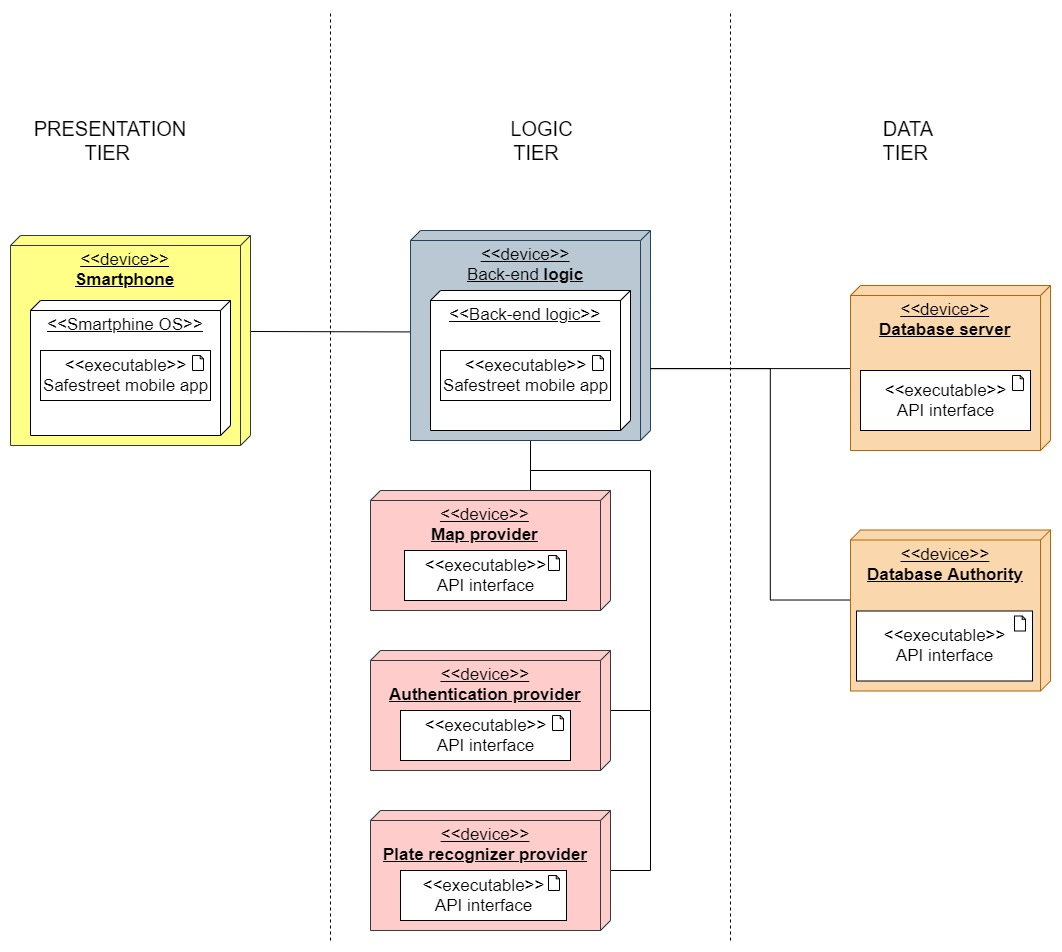
\includegraphics[scale = 1]{assets/deployment.png}\\[1.6 cm]
        %\caption[\textit{Deployment} Diagram]{Deployment diagram of the application.}
    \end{figure}
    This sequence diagram shows the process that allow a user to upload a new violation report.
    The information about the violation are send to the UserMobileApp, except for the position that is obtained by UserMobileApp throw the user device GPS\@.
    Then the database is queried to check if a violation with a similar date and time has already been reported.
    In that case, the NewReportManager send a request to the user to confirm the upload.
    If the answer is positive, or if a similar report has not been found at all, it uses all the collected information to create a dossier and store it in the database.
    Otherwise, if the user do not confirm the upload, the operation is aborted.
    \subsection{Daily Violation Map Request}\label{subsec:daily-violation-map-request}
    \begin{figure}[H]
        %\centering
        %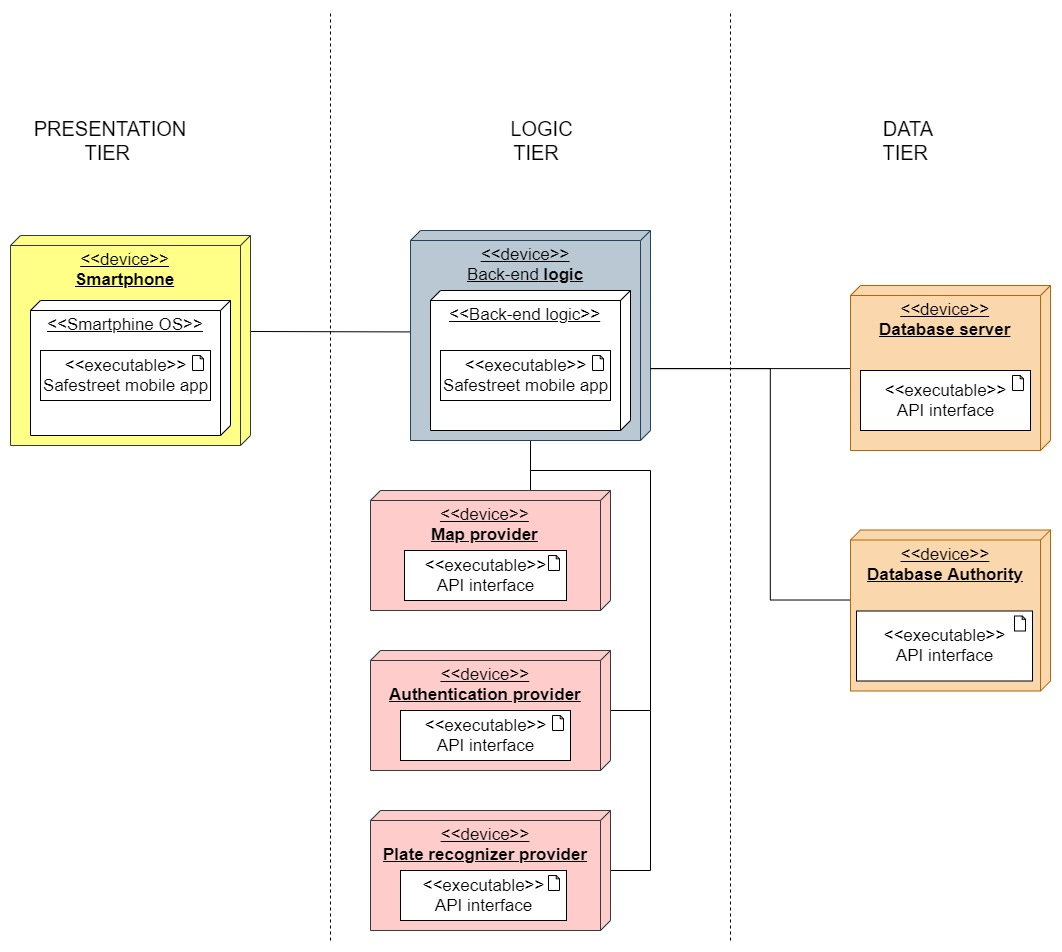
\includegraphics[scale = 1]{assets/deployment.png}\\[1.6 cm]
        %\caption[\textit{Deployment} Diagram]{Deployment diagram of the application.}
    \end{figure}
    In this sequence diagram is shown the process that provide to the user the daily violation map.
    It starts with a request from the user, that is followed with the collection of the collection of the information about the user position:
    this information is useful in order to set the map at the user location as default.
    Then the database is queried to collect all the report stored in the last 24 hours.
    Every report is than passed to the ReportMapManager,that mark the position of the report.
    The map thus obtained is than shown to the user.

    The sequence diagram shows than what happens in case that the user requires the dossier by clicking on the report marker:
    a request is sent from the UserMobileApp to the UserReportVisualizationManager, that uses the email to get the access level of the user and provides
    a dossier that contains only the accessible information.
    \subsection{Unsafe Area Request}\label{subsec:unsafe-area-request}
    \begin{figure}[H]
        %\centering
        %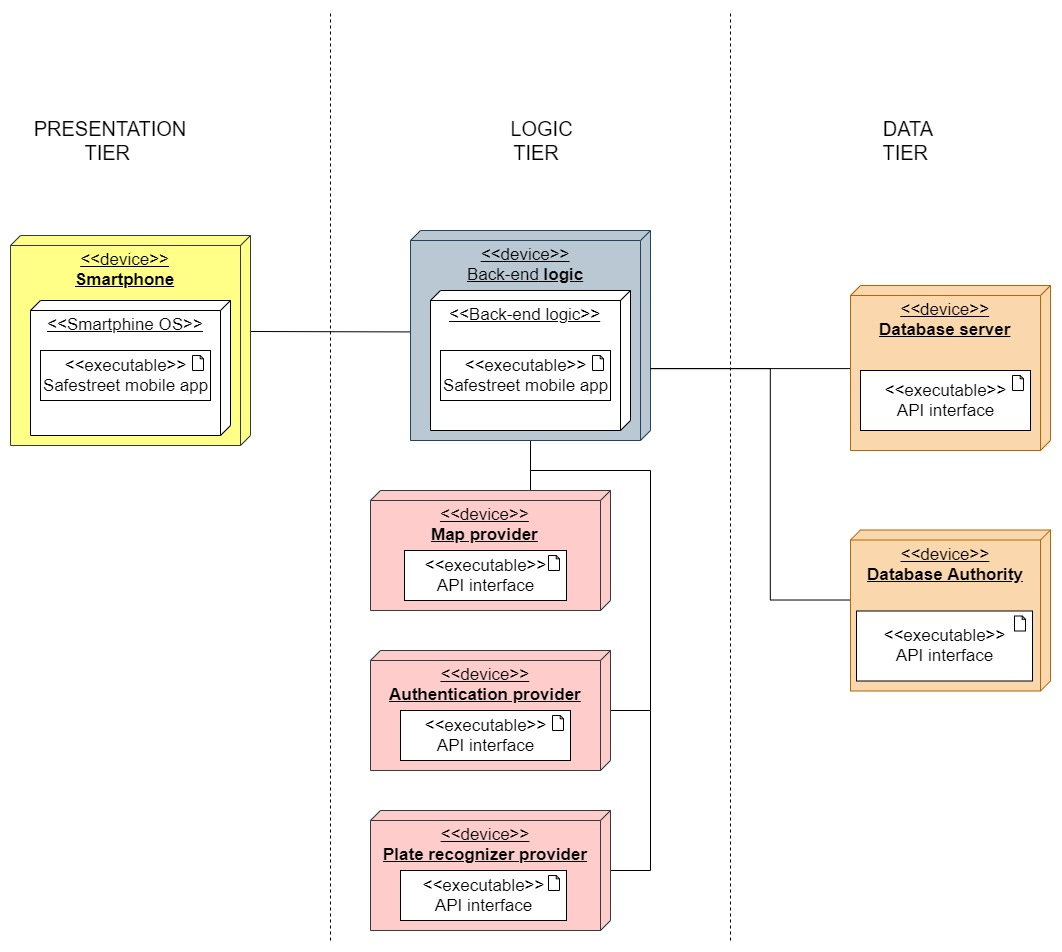
\includegraphics[scale = 1]{assets/deployment.png}\\[1.6 cm]
        %\caption[\textit{Deployment} Diagram]{Deployment diagram of the application.}
    \end{figure}
    This sequence diagram shows the process that provide the map of the unsafe are in a city,
    crossing the report collected by safe street and the accidents data provided by the local municipality.
    The user send a request, providing the location that would like to interrogate.
    The UserMobileApp send the request to the UnsafeAreaManager, which has the task of manage that kind of request.
    First, it get the accident list from the local municipality, and than get all the report collected into the indicated area.
    These information are than crossed and processed in order to define the unsafe areas, giving different weights to different type of violations.
    The data produced are than passed to the ReportMapManager, that mark the areas denoted as dangerous on the map.
    The map is then showed to the user.
    After that, the UnsafeAreaManager process the information on the violations and the accidents to find possible solutions,
    considering the type of the violations reported and the nearness of the accidents to the violations.
    If it is able to define possible solutions, these are send to the municipality.
    \subsection{Send Violation's picture Feedback}\label{subsec:send-violation's-picture-feedback}
    \begin{figure}[H]
        %\centering
        %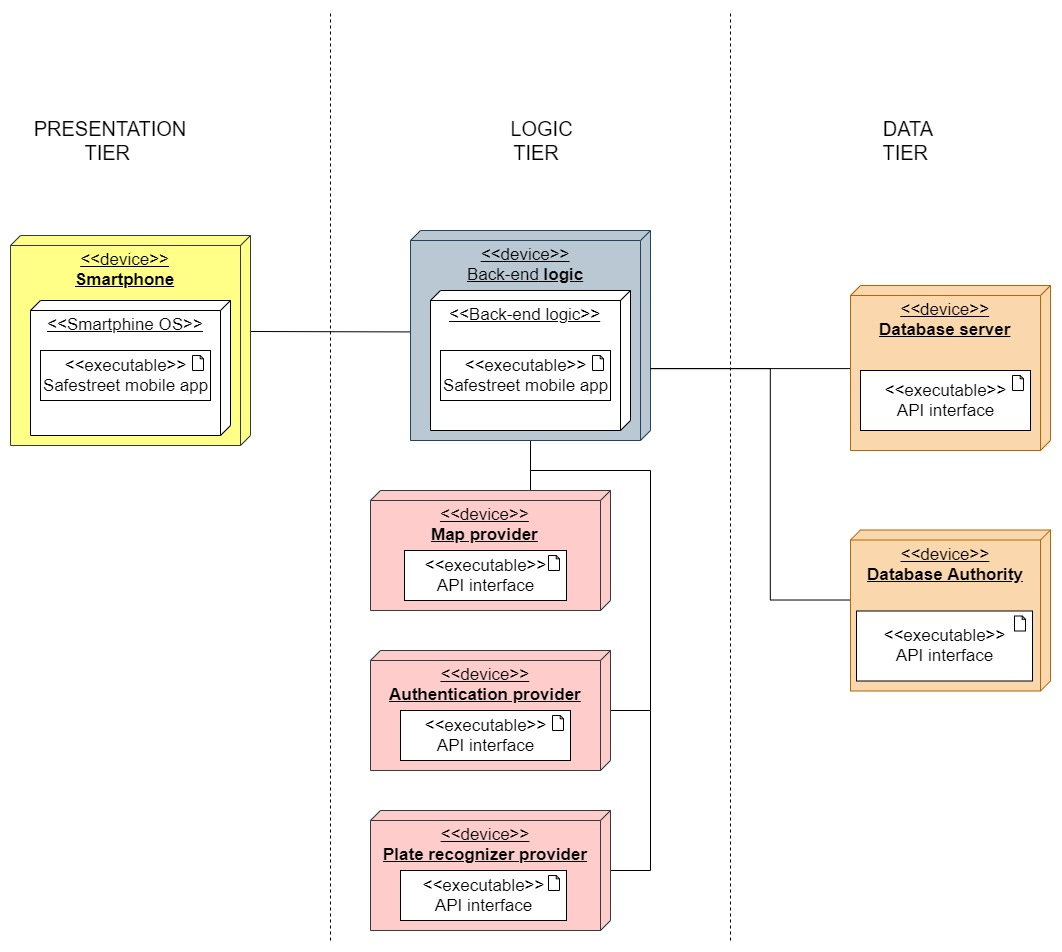
\includegraphics[scale = 1]{assets/deployment.png}\\[1.6 cm]
        %\caption[\textit{Deployment} Diagram]{Deployment diagram of the application.}
    \end{figure}
    This last sequence diagram show a situation in which a user give a feedback on a picture of a report.
    First, the user required the dossier of a report, that is provided to him by the UserReportVisualizationManager,
    that has the task to show him only the data that are allowed to his authorization level.
    Than, the user can decide to send a feedback of a picture: in that case, the information on the picture and the email of the user
    are send to the UserReportVisualizationManager, that first check if the picture has already a feedback associated to the user's email.
    If it already exist, the operation is aborted;
    otherwise, the reporting is accepted and different situations could occur.
    In the standard scenario, if the picture did not already have 5 reports, the feedback is just associated to the picture itself.
    Otherwise, if the picture had already collected 5 feedback, it is deleted from the dossier of the violation, deleting it from the database;
    now, if the violation has no more associated picture, it is entirely deleted from the database, since it has no more picture to validate the report.
    \newpage
    \section{Component Interfaces}\label{sec:component-interfaces}
    \begin{figure}[H]
        \centering
        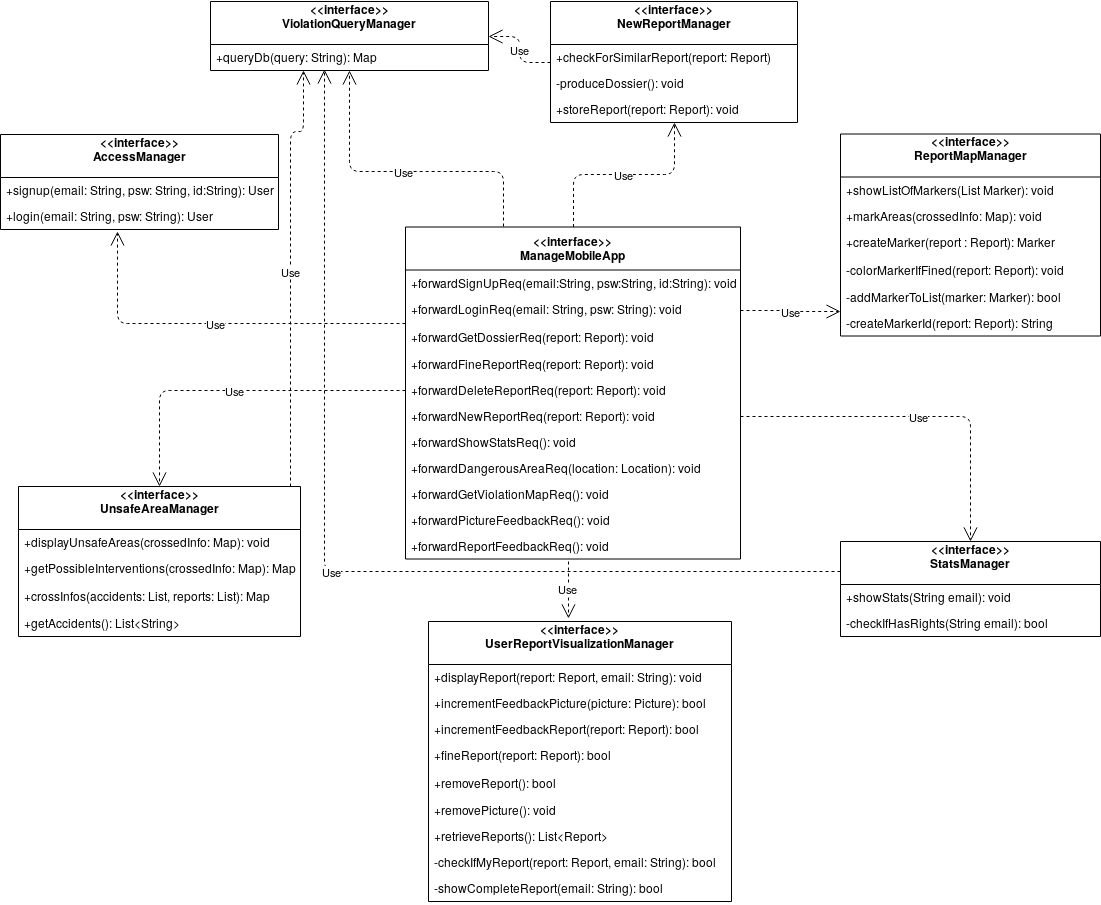
\includegraphics[scale = 0.45]{assets/interfaces.png}\\[1.6 cm]
        \caption[\textit{UML Interfaces} Diagram]{UML Interfaces diagram of the application.}
    \end{figure}
    All the methods below are not intended to be implemented as they are described, but their aim is to give a general idea of how the component
    interface will look like.
    Only the public methods of the managers are described.
    \\
    \\
    \textbf{AccessManager:}
    \begin{itemize}
        \item Function signup: given email, password and id(mandatory only if authority), a new instance of User is return by the authentication provider,
        and the new user is now stored in the database with its email and level(standard or complete, according to the id provided).
        \item Function login: given the email and password, will return a User object given by the authentication provider.
    \end{itemize}
    \textbf{NewReportManager:}
    \begin{itemize}
        \item     Function checkConstraintsOnReport: this function is used to check for example if at least one image is uploaded, will return true or false.
        \item     Function recognizePlates: given a list of images, the application will use an API in order to recognize plates text
        if present and will be put it in a list, one string for each image.
        \item     Function getPosition: this function will be called as soon as the first image is taken, will retrieve the user position using GPS.
        \item     Function checkForSimilarReports: this function will make sure that there are no other reports of the same violation in the same spot.
        \item     Function storeReport: the report will be then stored in the database, ready to be fetched by the other users.
        \item     Function getTime: this function will set the time of the report and will be taken from the device.
    \end{itemize}
    \textbf{ReportMapManager:}
    \begin{itemize}
        \item     Function showListOfMarkers: display all markers created on the map
        \item     Function addMarkerToList: given a report, the associated marker is created and return true if no errors occur.
        \item     Function markArea: once the crossed info between SafeStreet and the municipality are calculated, the most dangerous areas are marked.
    \end{itemize}
    \textbf{StatisticsManager:}
    \begin{itemize}
        \item     Function showStats: given the current user’s email that is logged, the right stats are loaded depending on the level of the user.
    \end{itemize}
    \textbf{UserReportVisualizationManager:}
    \begin{itemize}
        \item     Function displayReport: the report selected on the map will be shown, displaying partial or complete data (visible plates for example)
        depending on the level of the user.
        \item     Function incrementFeedbackReport: given a report, increment the counter of the negative feedback on that report.
        \item     Function incrementFeedbackPicture: given a picture inside a report, increment the counter of the negative feedback on that image.
        \item     Function sendFeedback: given a report, increment the counter of all feedback on that report.
        \item     Function fineReport: this method is available only for authorities, given a report will be marked as fined on the map.
        \item     Function removeReport: given a report, if that report belongs to the user who wants to perform that action, it will be deleted.
        Moreover, this function will also be called when the reports reaches the maximum number of negative feedback.
        \item     Function removePicture: when the maximum number of negative feedback on the single image is reached, the picture will be deleted.
        \item     Function retrieveReports: this method is called either once the map is loaded or whenever the user taps on the refresh button.
    \end{itemize}
    \textbf{UnsafeAreaManager:}
    \begin{itemize}
        \item     Function displayUnsafeAreas: given a map of information, all the unsafe areas will be displayed on the map
        \item     Function getPossibleInterventions: from the map of all crossed information received by the API of the municipality,
        the possible interventions are created according to a precise algorithm that compares the places of the accidents with the violation’s report
        in the same places.
    \end{itemize}
    \newpage
    \section{Selected Architectural Styles and Patterns}\label{sec:selected-architectural-styles-and-patterns}
    \subsection{Three Tier Architecture}\label{subsec:three-tier-architecture}
    As already mentioned in section 2.3, we chosen a multi-tiered architecture composed by three tiers: presentation, logic and data.
    The advantages of this choice are in terms of decoupling of the complexity of the system making him more flexible to future modification
    and in this way also more reusable.
    This division also provides more security to the system in fat it separates the access to data from the layer where then logic for presentation
    and for the interaction with the customer is located.
    \subsection{Serverless Approach}\label{subsec:serverless-approach}
    \begin{itemize}
        \item \textbf{Performance:} we want the database access to be fast and in order to do that could be useful to directly query it and get all the tuples locally.
        Moreover, using this approach the database has a local cache that stores query results for future use.
        When a client app issues a query, if the SDK determines that the cache contains up-to-date results for that query, the results can come directly from the cache.
        The obvious benefit here is that network bandwidth and latency are reduced.
        The results appear faster, even while offline, and the end user pays less data costs to see those results.
        If you make the request indirectly through a server, there is absolutely no client-side caching done by default.
        If you want to cache the results, you’ll have to do that on the client, using some mechanism you choose.
        \item \textbf{Price:} is tied (partly) to how much data the app reads.
        As mentioned previously, the local cache can prevent many data reads from happening on the server.
        Data coming from cache, unchanged on the server, prevents the cost of the query and the cost of the bandwidth to bring that data to the app.
        If you query indirectly through a server in the middle, you will pay for the cost of the query in addition to the cost of the execution of the function.
        Usually the server SDKs you use do not cache data, so each execution pays the full cost of the query, and its data transfer.
    \end{itemize}

    \subsection{MVVM (Model-View-ViewModel)}\label{subsec:mvvmmodel-view-viewmodel}
    MVVM facilitates a separation of development of the graphical user interface - be it via a markup language or GUI code -
    from development of the business logic or back-end logic (the data model).
    The view model of MVVM is a value converter, meaning the view model is responsible for exposing (converting) the data objects from the model
    in such a way that objects are easily managed and presented.
    In this respect, the view model is more model than view, and handles most if not all of the view's display logic.
    Unlike the controller method (MVC pattern), the ViewModel method (MVVM) relies heavily on the frontend of the application.
    ViewModel acts as a binder that binds data between the view and model.
    Whereas the MVC format is specifically designed to create a separation of concerns between the model and view,
    the MVVM format with data-binding is designed specifically to allow the view and model to communicate directly with each other.
    This is why single page applications work very well with ViewModels.
    It’s simple and allows the view to directly communicate with the backend.
    Because of this, MVVM single page applications can move quickly and fluidly and save information to the database continuously
    (Google Docs would be a perfect example).

    \subsection{RESTful Architecture}\label{subsec:restful-architecture}
    The communication between SafeStreets and their users is done via HTTP requests following REST principles.
    REST (Representation State Transfer) is an architectural style for communication based on strict use of HTTP request types.
    One of the most important REST principles is that the interaction between the client and server is stateless between requests.
    Each request from the client to the server must contain all of the information necessary to understand the request.
    The client would not notice if the server were to be restarted at any point between the requests.
    The RESTful HTTP requests are categorized according to method types as the following:
    \begin{itemize}
        \item GET: used to retrieve resource representation/information only - and not to modify it in any way.
        \item POST: used to create a new resource into the collection of resources.
        \item PUT: used primarily to update existing resource (if the resource does not exist
        then API may decide to create a new resource or not).
        \item DELETE: used to delete resources (identified by the Request-URI).
    \end{itemize}
    \newpage
    \section{Other Design Decisions}\label{sec:other-design-decisions}
    \textbf{Choice of Providers} \\
    Starting from security and scalability reason, we have decided to lean on different providers for the more complexes and sensitives functionalities of SafeStreets.
    \begin{itemize}
        \item \textbf{Authentication Provider:} Regarding the authentication provider we want a service that can: \begin{enumerate}
                                                                                                                     \item Register new users
                                                                                                                     \item Authenticate the registered ones
                                                                                                                 \end{enumerate}
        The best effort is the encryption of the password that is useful in terms of security.
        \item \textbf{Map Provider:} It's fundamental in SafeStreets app for display report on a map.
        Furthermore the map provider must be able to displays the position of the user and of the reports on the map.
        \item \textbf{Plate Recognizer Provider:} For recognize a plate from a picture, we decide to choose a provider that it’s be able from a photo
        to keep the plate (text format).
        \item \textbf{Database Provider:} Database system are complex, difficult and time-consuming to design also for the developers
        requires an initial training so from this point of view is more convenient to take one ready-made.
        We want a database that stores reports with all their information and also be able to retrieve information about one user from his mail.
    \end{itemize}

\end{document}